\documentclass[pdftex,12pt,a4paper]{article}
\usepackage[pdftex]{graphicx}

\title{Updating TOPLATS with Fortran 2003}
\author{\\ \\ Nathaniel Chaney\\ Colby Fisher\\ Amanda Siemann\\ Ruolan Xu\\ Wang Zhan \\ \\ Department of Civil and Environmental Engineering}
\date{}
%\date{January 14, 2013}                                           % Activate to display a given date or no date

\begin{document}

\maketitle
\vfill
\begin{center}
{\large \today}
\end{center}

\newpage
\section{Introduction}
{(Effi)}
{\\ Introduce TOPLATS, our motivation and goals (adapted from design document)}

\section{Interface}
{(Nate)}
{\\ Driver}
{\\ Separate I/O from actual model}
{\\ Simplified input files}

\section{Modularization}
One of the tasks in the project is modularization. We set up 11 modules for the model and split tests from its own interface. Each module is written in a separate file. By modularization, we are able to reduce the total number of files from more than 50 to 11. The new TOPLATS model files are shown in Figure \ref{Modules1}. The model are consist of two main parts: MODULE\_CELL and MODULE\_CATCHMENT. MODULE\_CELL uses MODULE\_LAND, MODULE\_ATMOS, MODULE\_CANOPY and MODULE\_SNOW. The program IO is separated into MODULE\_IO and variables and data structures defined in MODULE\_VARIABLES. With modularization, swapping physics in the model becomes much easier since we are able to replace the subroutine or module instead of making changes to every related variables and functions throughout the model.

\begin{figure}[h]
	\centering
	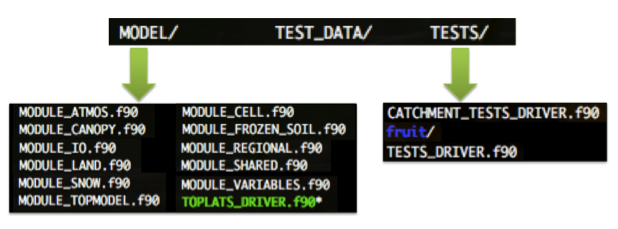
\includegraphics[width=4.5in]{Figures/Modules1.png}
	\label{Modules1}
	\caption{New TOPLATS model}
\end{figure}

\begin{figure}[h]
	\centering
	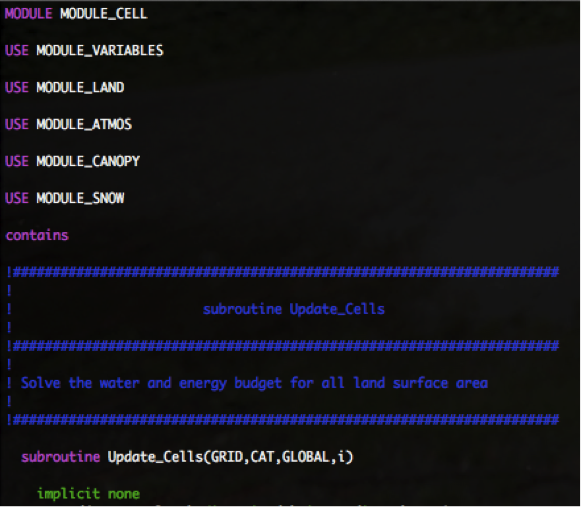
\includegraphics[width=4.5in]{Figures/Modules2.png}
	\label{Modules2}
	\caption{Snapshot of MODULE\_CELL.f90}
\end{figure}

Within each module, as shown in Figure \ref{Modules2}, we first listed shared variables and structures from other modules, defined structures being shared by subroutines in the module if there is any, and then listed the subroutines that are related to the module. Routines are being regrouped by their function. 

\section{Variables}
In the original version of TOPLATS, the variables were stored in one lengthy list. As previously mentioned, the hundreds of variables were passed into subroutines individually, causing extremely large subroutine calls. For the updated version of TOPLATS developed in this project, these hundreds of variables were organized into derived data types (structures) based upon function or purpose. In this way, structures could be passed into the modules and subroutines in relevant groups, thereby cleaning up the otherwise unmanageable code. In each larger subroutine, such as Atmos, the variables used in the code were replaced with the corresponding member of the structure. For each smaller subroutine, the members of the structures were passed into the subroutine individually to avoid passing in more variables than necessary.

Not only was the original version of TOPLATS crippled by the massive subroutine calls, but it was also impaired by the unreasonable number of help files storing the initialized variables with their corresponding types. Each subroutine was associated with a help file which initialized new variables in each subroutine but which also re-initialized all variables which were passed into the subroutine. This process of re-initializing variables over and over was cumbersome and unnecessary. In the updated version of TOPLATS, the variables in structures are initialized within the structure, and the rest of the variables are only initialized within the larger subroutine in which they are used. In this way, hundreds of files were removed.

Another limitation of the original version of TOPLATS was the use of static memory allocation. Using this method, the size of all arrays needed to be provided at compile time, meaning that the users needed to alter the source files every time they used the model for a different domain. In order to improve upon this, the dynamic memory allocation features implemented in Fortran 90 were used. By dynamically allocating the arrays, the user is able to specify dimensions at run time, allowing for the model to be used across multiple domains without maintaining and compiling multiple versions of the model code.

\section{Tests}
{(Effi)}
{\\ Catchment tests\\ Unit tests on subroutines}

\section{Parallelization}
Parallelization is currently implemented using OpenMP and uses up to 8 cores on a single node, depending on the preference of the user.  In order to do this, the domain is split up into equal sized blocks and then is distributed among the threads. Calculations are then performed for each cell before the domain is reassembled and the regional processes are calculated. For the domain size that we are using the parallelization does not have a significant impact on the calculation time. It should be noted though that for future work, as the domain size increases, we believe that we will find that parallelization becomes increasingly important. In order to run the model on a global scale, we plan to implement parallelization through MPI in order to maximize the computational power of each node.



\section{Valgrind}
{(Colby)}
{\\ Valgrind detects uninitialized variables}

\section{Profiling}

\begin{figure}[h]
	%\centering
	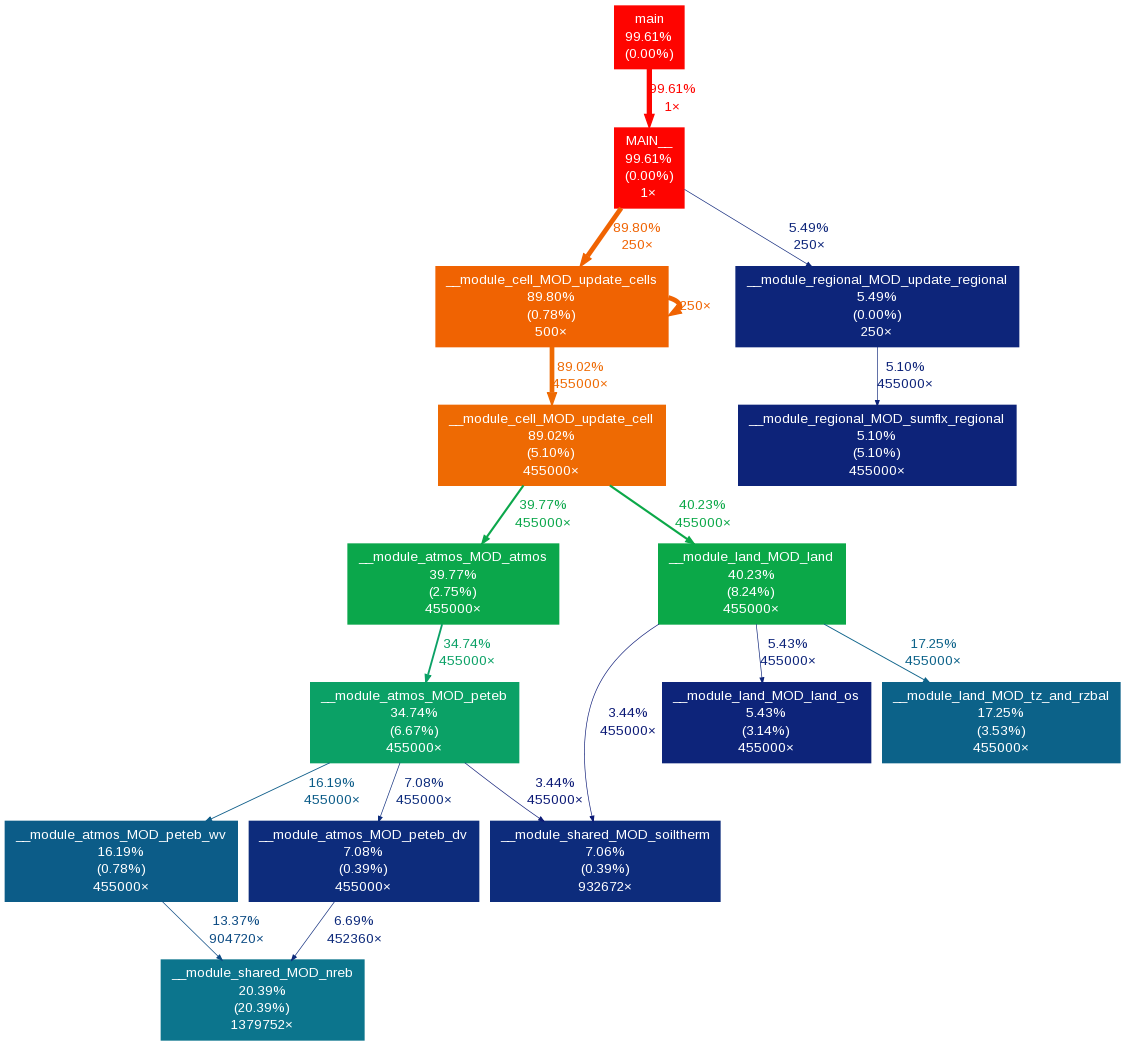
\includegraphics[width=5.5in]{Figures/CallGraph.png}
	\label{Profiling1}
	\caption{}
\end{figure}

\section{Conclusion}
{(Effi)}
{Lessons learned e.g. version control and github helps collaboration}
{ \\ Future developement}
\end{document}